% Created by tikzDevice version 0.12.3.1 on 2021-03-12 12:08:22
% !TEX encoding = UTF-8 Unicode
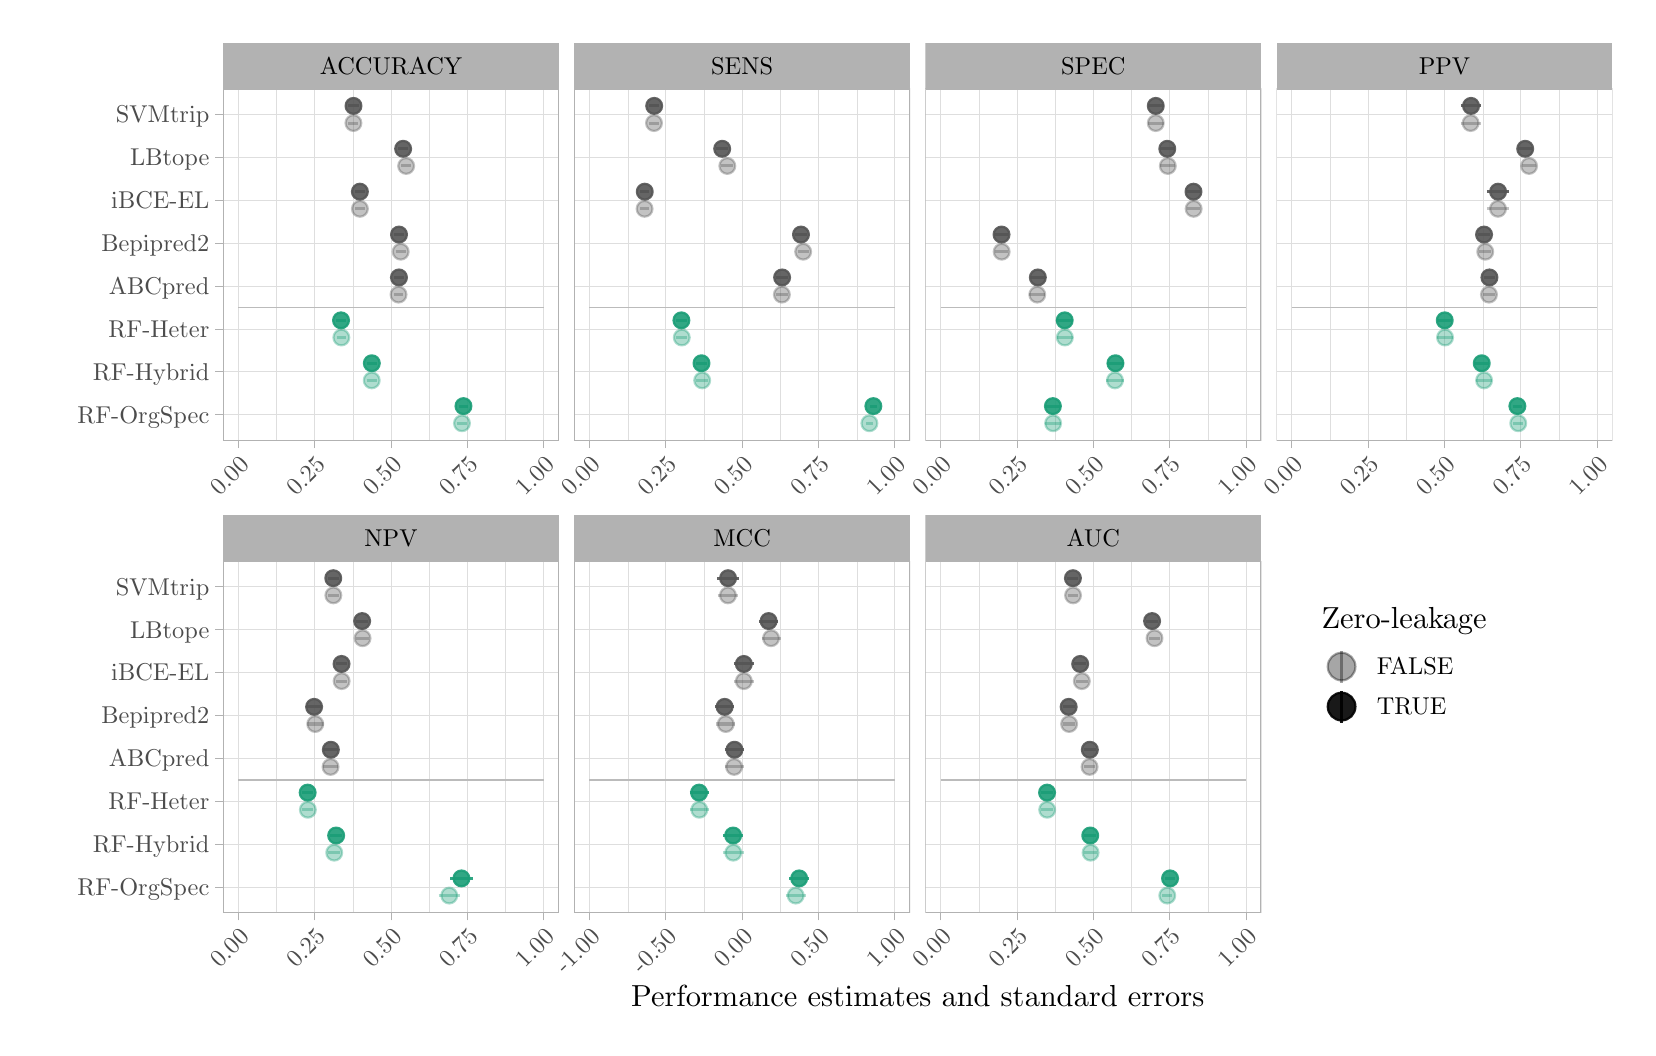
\begin{tikzpicture}[x=1pt,y=1pt]
\definecolor{fillColor}{RGB}{255,255,255}
\path[use as bounding box,fill=fillColor,fill opacity=0.00] (0,0) rectangle (578.16,361.35);
\begin{scope}
\path[clip] (  0.00,  0.00) rectangle (578.16,361.35);
\definecolor{drawColor}{RGB}{255,255,255}
\definecolor{fillColor}{RGB}{255,255,255}

\path[draw=drawColor,line width= 0.6pt,line join=round,line cap=round,fill=fillColor] (  0.00,  0.00) rectangle (578.16,361.35);
\end{scope}
\begin{scope}
\path[clip] ( 70.59,212.20) rectangle (191.99,339.28);
\definecolor{fillColor}{RGB}{255,255,255}

\path[fill=fillColor] ( 70.59,212.20) rectangle (191.99,339.28);
\definecolor{drawColor}{gray}{0.87}

\path[draw=drawColor,line width= 0.1pt,line join=round] ( 89.91,212.20) --
	( 89.91,339.28);

\path[draw=drawColor,line width= 0.1pt,line join=round] (117.50,212.20) --
	(117.50,339.28);

\path[draw=drawColor,line width= 0.1pt,line join=round] (145.08,212.20) --
	(145.08,339.28);

\path[draw=drawColor,line width= 0.1pt,line join=round] (172.67,212.20) --
	(172.67,339.28);

\path[draw=drawColor,line width= 0.3pt,line join=round] ( 70.59,221.50) --
	(191.99,221.50);

\path[draw=drawColor,line width= 0.3pt,line join=round] ( 70.59,236.99) --
	(191.99,236.99);

\path[draw=drawColor,line width= 0.3pt,line join=round] ( 70.59,252.49) --
	(191.99,252.49);

\path[draw=drawColor,line width= 0.3pt,line join=round] ( 70.59,267.99) --
	(191.99,267.99);

\path[draw=drawColor,line width= 0.3pt,line join=round] ( 70.59,283.49) --
	(191.99,283.49);

\path[draw=drawColor,line width= 0.3pt,line join=round] ( 70.59,298.98) --
	(191.99,298.98);

\path[draw=drawColor,line width= 0.3pt,line join=round] ( 70.59,314.48) --
	(191.99,314.48);

\path[draw=drawColor,line width= 0.3pt,line join=round] ( 70.59,329.98) --
	(191.99,329.98);

\path[draw=drawColor,line width= 0.3pt,line join=round] ( 76.11,212.20) --
	( 76.11,339.28);

\path[draw=drawColor,line width= 0.3pt,line join=round] (103.70,212.20) --
	(103.70,339.28);

\path[draw=drawColor,line width= 0.3pt,line join=round] (131.29,212.20) --
	(131.29,339.28);

\path[draw=drawColor,line width= 0.3pt,line join=round] (158.88,212.20) --
	(158.88,339.28);

\path[draw=drawColor,line width= 0.3pt,line join=round] (186.47,212.20) --
	(186.47,339.28);
\definecolor{drawColor}{RGB}{27,158,119}

\path[draw=drawColor,draw opacity=0.35,line width= 1.1pt,line join=round] (155.28,218.40) -- (158.59,218.40);

\path[draw=drawColor,draw opacity=0.35,line width= 1.1pt,line join=round] (122.51,233.90) -- (126.14,233.90);

\path[draw=drawColor,draw opacity=0.35,line width= 1.1pt,line join=round] (111.70,249.39) -- (114.98,249.39);
\definecolor{drawColor}{RGB}{85,85,85}

\path[draw=drawColor,draw opacity=0.35,line width= 1.1pt,line join=round] (132.30,264.89) -- (135.73,264.89);

\path[draw=drawColor,draw opacity=0.35,line width= 1.1pt,line join=round] (133.00,280.39) -- (136.59,280.39);

\path[draw=drawColor,draw opacity=0.35,line width= 1.1pt,line join=round] (118.25,295.89) -- (121.85,295.89);

\path[draw=drawColor,draw opacity=0.35,line width= 1.1pt,line join=round] (134.98,311.38) -- (138.54,311.38);

\path[draw=drawColor,draw opacity=0.35,line width= 1.1pt,line join=round] (115.92,326.88) -- (119.50,326.88);
\definecolor{drawColor}{RGB}{85,85,85}

\path[draw=drawColor,draw opacity=0.90,line width= 1.1pt,line join=round] (132.34,271.09) -- (135.98,271.09);

\path[draw=drawColor,draw opacity=0.90,line width= 1.1pt,line join=round] (132.39,286.59) -- (135.97,286.59);

\path[draw=drawColor,draw opacity=0.90,line width= 1.1pt,line join=round] (118.27,302.08) -- (121.81,302.08);

\path[draw=drawColor,draw opacity=0.90,line width= 1.1pt,line join=round] (133.85,317.58) -- (137.50,317.58);

\path[draw=drawColor,draw opacity=0.90,line width= 1.1pt,line join=round] (115.90,333.08) -- (119.56,333.08);
\definecolor{drawColor}{RGB}{27,158,119}

\path[draw=drawColor,draw opacity=0.90,line width= 1.1pt,line join=round] (155.89,224.60) -- (159.05,224.60);

\path[draw=drawColor,draw opacity=0.90,line width= 1.1pt,line join=round] (122.62,240.09) -- (126.11,240.09);

\path[draw=drawColor,draw opacity=0.90,line width= 1.1pt,line join=round] (111.58,255.59) -- (114.88,255.59);
\definecolor{drawColor}{RGB}{27,158,119}
\definecolor{fillColor}{RGB}{27,158,119}

\path[draw=drawColor,draw opacity=0.35,line width= 0.8pt,line join=round,line cap=round,fill=fillColor,fill opacity=0.35] (156.93,218.40) circle (  2.85);

\path[draw=drawColor,draw opacity=0.35,line width= 0.8pt,line join=round,line cap=round,fill=fillColor,fill opacity=0.35] (124.32,233.90) circle (  2.85);

\path[draw=drawColor,draw opacity=0.35,line width= 0.8pt,line join=round,line cap=round,fill=fillColor,fill opacity=0.35] (113.34,249.39) circle (  2.85);
\definecolor{drawColor}{RGB}{85,85,85}
\definecolor{fillColor}{RGB}{85,85,85}

\path[draw=drawColor,draw opacity=0.35,line width= 0.8pt,line join=round,line cap=round,fill=fillColor,fill opacity=0.35] (134.01,264.89) circle (  2.85);

\path[draw=drawColor,draw opacity=0.35,line width= 0.8pt,line join=round,line cap=round,fill=fillColor,fill opacity=0.35] (134.79,280.39) circle (  2.85);

\path[draw=drawColor,draw opacity=0.35,line width= 0.8pt,line join=round,line cap=round,fill=fillColor,fill opacity=0.35] (120.05,295.89) circle (  2.85);

\path[draw=drawColor,draw opacity=0.35,line width= 0.8pt,line join=round,line cap=round,fill=fillColor,fill opacity=0.35] (136.76,311.38) circle (  2.85);

\path[draw=drawColor,draw opacity=0.35,line width= 0.8pt,line join=round,line cap=round,fill=fillColor,fill opacity=0.35] (117.71,326.88) circle (  2.85);
\definecolor{drawColor}{RGB}{85,85,85}
\definecolor{fillColor}{RGB}{85,85,85}

\path[draw=drawColor,draw opacity=0.90,line width= 0.8pt,line join=round,line cap=round,fill=fillColor,fill opacity=0.90] (134.16,271.09) circle (  2.85);

\path[draw=drawColor,draw opacity=0.90,line width= 0.8pt,line join=round,line cap=round,fill=fillColor,fill opacity=0.90] (134.18,286.59) circle (  2.85);

\path[draw=drawColor,draw opacity=0.90,line width= 0.8pt,line join=round,line cap=round,fill=fillColor,fill opacity=0.90] (120.04,302.08) circle (  2.85);

\path[draw=drawColor,draw opacity=0.90,line width= 0.8pt,line join=round,line cap=round,fill=fillColor,fill opacity=0.90] (135.67,317.58) circle (  2.85);

\path[draw=drawColor,draw opacity=0.90,line width= 0.8pt,line join=round,line cap=round,fill=fillColor,fill opacity=0.90] (117.73,333.08) circle (  2.85);
\definecolor{drawColor}{RGB}{27,158,119}
\definecolor{fillColor}{RGB}{27,158,119}

\path[draw=drawColor,draw opacity=0.90,line width= 0.8pt,line join=round,line cap=round,fill=fillColor,fill opacity=0.90] (157.47,224.60) circle (  2.85);

\path[draw=drawColor,draw opacity=0.90,line width= 0.8pt,line join=round,line cap=round,fill=fillColor,fill opacity=0.90] (124.36,240.09) circle (  2.85);

\path[draw=drawColor,draw opacity=0.90,line width= 0.8pt,line join=round,line cap=round,fill=fillColor,fill opacity=0.90] (113.23,255.59) circle (  2.85);
\definecolor{drawColor}{RGB}{187,187,187}

\path[draw=drawColor,line width= 0.6pt,line join=round] ( 76.11,260.24) -- (186.47,260.24);
\definecolor{drawColor}{gray}{0.70}

\path[draw=drawColor,line width= 0.6pt,line join=round,line cap=round] ( 70.59,212.20) rectangle (191.99,339.28);
\end{scope}
\begin{scope}
\path[clip] ( 70.59, 41.54) rectangle (191.99,168.62);
\definecolor{fillColor}{RGB}{255,255,255}

\path[fill=fillColor] ( 70.59, 41.54) rectangle (191.99,168.62);
\definecolor{drawColor}{gray}{0.87}

\path[draw=drawColor,line width= 0.1pt,line join=round] ( 89.91, 41.54) --
	( 89.91,168.62);

\path[draw=drawColor,line width= 0.1pt,line join=round] (117.50, 41.54) --
	(117.50,168.62);

\path[draw=drawColor,line width= 0.1pt,line join=round] (145.08, 41.54) --
	(145.08,168.62);

\path[draw=drawColor,line width= 0.1pt,line join=round] (172.67, 41.54) --
	(172.67,168.62);

\path[draw=drawColor,line width= 0.3pt,line join=round] ( 70.59, 50.84) --
	(191.99, 50.84);

\path[draw=drawColor,line width= 0.3pt,line join=round] ( 70.59, 66.34) --
	(191.99, 66.34);

\path[draw=drawColor,line width= 0.3pt,line join=round] ( 70.59, 81.84) --
	(191.99, 81.84);

\path[draw=drawColor,line width= 0.3pt,line join=round] ( 70.59, 97.33) --
	(191.99, 97.33);

\path[draw=drawColor,line width= 0.3pt,line join=round] ( 70.59,112.83) --
	(191.99,112.83);

\path[draw=drawColor,line width= 0.3pt,line join=round] ( 70.59,128.33) --
	(191.99,128.33);

\path[draw=drawColor,line width= 0.3pt,line join=round] ( 70.59,143.83) --
	(191.99,143.83);

\path[draw=drawColor,line width= 0.3pt,line join=round] ( 70.59,159.32) --
	(191.99,159.32);

\path[draw=drawColor,line width= 0.3pt,line join=round] ( 76.11, 41.54) --
	( 76.11,168.62);

\path[draw=drawColor,line width= 0.3pt,line join=round] (103.70, 41.54) --
	(103.70,168.62);

\path[draw=drawColor,line width= 0.3pt,line join=round] (131.29, 41.54) --
	(131.29,168.62);

\path[draw=drawColor,line width= 0.3pt,line join=round] (158.88, 41.54) --
	(158.88,168.62);

\path[draw=drawColor,line width= 0.3pt,line join=round] (186.47, 41.54) --
	(186.47,168.62);
\definecolor{drawColor}{RGB}{27,158,119}

\path[draw=drawColor,draw opacity=0.35,line width= 1.1pt,line join=round] (148.45, 47.74) -- (156.22, 47.74);

\path[draw=drawColor,draw opacity=0.35,line width= 1.1pt,line join=round] (108.57, 63.24) -- (112.97, 63.24);

\path[draw=drawColor,draw opacity=0.35,line width= 1.1pt,line join=round] ( 99.30, 78.74) -- (103.20, 78.74);
\definecolor{drawColor}{RGB}{85,85,85}

\path[draw=drawColor,draw opacity=0.35,line width= 1.1pt,line join=round] (106.62, 94.23) -- (112.25, 94.23);

\path[draw=drawColor,draw opacity=0.35,line width= 1.1pt,line join=round] (100.90,109.73) -- (106.91,109.73);

\path[draw=drawColor,draw opacity=0.35,line width= 1.1pt,line join=round] (111.52,125.23) -- (115.39,125.23);

\path[draw=drawColor,draw opacity=0.35,line width= 1.1pt,line join=round] (118.74,140.73) -- (123.27,140.73);

\path[draw=drawColor,draw opacity=0.35,line width= 1.1pt,line join=round] (108.47,156.22) -- (112.44,156.22);
\definecolor{drawColor}{RGB}{85,85,85}

\path[draw=drawColor,draw opacity=0.90,line width= 1.1pt,line join=round] (106.84,100.43) -- (112.27,100.43);

\path[draw=drawColor,draw opacity=0.90,line width= 1.1pt,line join=round] (100.51,115.93) -- (106.49,115.93);

\path[draw=drawColor,draw opacity=0.90,line width= 1.1pt,line join=round] (111.51,131.43) -- (115.31,131.43);

\path[draw=drawColor,draw opacity=0.90,line width= 1.1pt,line join=round] (118.62,146.93) -- (123.11,146.93);

\path[draw=drawColor,draw opacity=0.90,line width= 1.1pt,line join=round] (108.46,162.42) -- (112.39,162.42);
\definecolor{drawColor}{RGB}{27,158,119}

\path[draw=drawColor,draw opacity=0.90,line width= 1.1pt,line join=round] (152.69, 53.94) -- (160.78, 53.94);

\path[draw=drawColor,draw opacity=0.90,line width= 1.1pt,line join=round] (109.28, 69.44) -- (113.65, 69.44);

\path[draw=drawColor,draw opacity=0.90,line width= 1.1pt,line join=round] ( 99.24, 84.94) -- (103.09, 84.94);
\definecolor{drawColor}{RGB}{27,158,119}
\definecolor{fillColor}{RGB}{27,158,119}

\path[draw=drawColor,draw opacity=0.35,line width= 0.8pt,line join=round,line cap=round,fill=fillColor,fill opacity=0.35] (152.33, 47.74) circle (  2.85);

\path[draw=drawColor,draw opacity=0.35,line width= 0.8pt,line join=round,line cap=round,fill=fillColor,fill opacity=0.35] (110.77, 63.24) circle (  2.85);

\path[draw=drawColor,draw opacity=0.35,line width= 0.8pt,line join=round,line cap=round,fill=fillColor,fill opacity=0.35] (101.25, 78.74) circle (  2.85);
\definecolor{drawColor}{RGB}{85,85,85}
\definecolor{fillColor}{RGB}{85,85,85}

\path[draw=drawColor,draw opacity=0.35,line width= 0.8pt,line join=round,line cap=round,fill=fillColor,fill opacity=0.35] (109.44, 94.23) circle (  2.85);

\path[draw=drawColor,draw opacity=0.35,line width= 0.8pt,line join=round,line cap=round,fill=fillColor,fill opacity=0.35] (103.91,109.73) circle (  2.85);

\path[draw=drawColor,draw opacity=0.35,line width= 0.8pt,line join=round,line cap=round,fill=fillColor,fill opacity=0.35] (113.45,125.23) circle (  2.85);

\path[draw=drawColor,draw opacity=0.35,line width= 0.8pt,line join=round,line cap=round,fill=fillColor,fill opacity=0.35] (121.01,140.73) circle (  2.85);

\path[draw=drawColor,draw opacity=0.35,line width= 0.8pt,line join=round,line cap=round,fill=fillColor,fill opacity=0.35] (110.46,156.22) circle (  2.85);
\definecolor{drawColor}{RGB}{85,85,85}
\definecolor{fillColor}{RGB}{85,85,85}

\path[draw=drawColor,draw opacity=0.90,line width= 0.8pt,line join=round,line cap=round,fill=fillColor,fill opacity=0.90] (109.55,100.43) circle (  2.85);

\path[draw=drawColor,draw opacity=0.90,line width= 0.8pt,line join=round,line cap=round,fill=fillColor,fill opacity=0.90] (103.50,115.93) circle (  2.85);

\path[draw=drawColor,draw opacity=0.90,line width= 0.8pt,line join=round,line cap=round,fill=fillColor,fill opacity=0.90] (113.41,131.43) circle (  2.85);

\path[draw=drawColor,draw opacity=0.90,line width= 0.8pt,line join=round,line cap=round,fill=fillColor,fill opacity=0.90] (120.86,146.93) circle (  2.85);

\path[draw=drawColor,draw opacity=0.90,line width= 0.8pt,line join=round,line cap=round,fill=fillColor,fill opacity=0.90] (110.42,162.42) circle (  2.85);
\definecolor{drawColor}{RGB}{27,158,119}
\definecolor{fillColor}{RGB}{27,158,119}

\path[draw=drawColor,draw opacity=0.90,line width= 0.8pt,line join=round,line cap=round,fill=fillColor,fill opacity=0.90] (156.74, 53.94) circle (  2.85);

\path[draw=drawColor,draw opacity=0.90,line width= 0.8pt,line join=round,line cap=round,fill=fillColor,fill opacity=0.90] (111.47, 69.44) circle (  2.85);

\path[draw=drawColor,draw opacity=0.90,line width= 0.8pt,line join=round,line cap=round,fill=fillColor,fill opacity=0.90] (101.17, 84.94) circle (  2.85);
\definecolor{drawColor}{RGB}{187,187,187}

\path[draw=drawColor,line width= 0.6pt,line join=round] ( 76.11, 89.59) -- (186.47, 89.59);
\definecolor{drawColor}{gray}{0.70}

\path[draw=drawColor,line width= 0.6pt,line join=round,line cap=round] ( 70.59, 41.54) rectangle (191.99,168.62);
\end{scope}
\begin{scope}
\path[clip] (197.49,212.20) rectangle (318.88,339.28);
\definecolor{fillColor}{RGB}{255,255,255}

\path[fill=fillColor] (197.49,212.20) rectangle (318.88,339.28);
\definecolor{drawColor}{gray}{0.87}

\path[draw=drawColor,line width= 0.1pt,line join=round] (216.80,212.20) --
	(216.80,339.28);

\path[draw=drawColor,line width= 0.1pt,line join=round] (244.39,212.20) --
	(244.39,339.28);

\path[draw=drawColor,line width= 0.1pt,line join=round] (271.98,212.20) --
	(271.98,339.28);

\path[draw=drawColor,line width= 0.1pt,line join=round] (299.56,212.20) --
	(299.56,339.28);

\path[draw=drawColor,line width= 0.3pt,line join=round] (197.49,221.50) --
	(318.88,221.50);

\path[draw=drawColor,line width= 0.3pt,line join=round] (197.49,236.99) --
	(318.88,236.99);

\path[draw=drawColor,line width= 0.3pt,line join=round] (197.49,252.49) --
	(318.88,252.49);

\path[draw=drawColor,line width= 0.3pt,line join=round] (197.49,267.99) --
	(318.88,267.99);

\path[draw=drawColor,line width= 0.3pt,line join=round] (197.49,283.49) --
	(318.88,283.49);

\path[draw=drawColor,line width= 0.3pt,line join=round] (197.49,298.98) --
	(318.88,298.98);

\path[draw=drawColor,line width= 0.3pt,line join=round] (197.49,314.48) --
	(318.88,314.48);

\path[draw=drawColor,line width= 0.3pt,line join=round] (197.49,329.98) --
	(318.88,329.98);

\path[draw=drawColor,line width= 0.3pt,line join=round] (203.00,212.20) --
	(203.00,339.28);

\path[draw=drawColor,line width= 0.3pt,line join=round] (230.59,212.20) --
	(230.59,339.28);

\path[draw=drawColor,line width= 0.3pt,line join=round] (258.18,212.20) --
	(258.18,339.28);

\path[draw=drawColor,line width= 0.3pt,line join=round] (285.77,212.20) --
	(285.77,339.28);

\path[draw=drawColor,line width= 0.3pt,line join=round] (313.36,212.20) --
	(313.36,339.28);
\definecolor{drawColor}{RGB}{27,158,119}

\path[draw=drawColor,draw opacity=0.35,line width= 1.1pt,line join=round] (302.93,218.40) -- (305.37,218.40);

\path[draw=drawColor,draw opacity=0.35,line width= 1.1pt,line join=round] (241.61,233.90) -- (245.86,233.90);

\path[draw=drawColor,draw opacity=0.35,line width= 1.1pt,line join=round] (234.43,249.39) -- (238.29,249.39);
\definecolor{drawColor}{RGB}{85,85,85}

\path[draw=drawColor,draw opacity=0.35,line width= 1.1pt,line join=round] (270.47,264.89) -- (274.58,264.89);

\path[draw=drawColor,draw opacity=0.35,line width= 1.1pt,line join=round] (278.22,280.39) -- (282.21,280.39);

\path[draw=drawColor,draw opacity=0.35,line width= 1.1pt,line join=round] (221.21,295.89) -- (224.63,295.89);

\path[draw=drawColor,draw opacity=0.35,line width= 1.1pt,line join=round] (250.60,311.38) -- (255.02,311.38);

\path[draw=drawColor,draw opacity=0.35,line width= 1.1pt,line join=round] (224.56,326.88) -- (228.07,326.88);
\definecolor{drawColor}{RGB}{85,85,85}

\path[draw=drawColor,draw opacity=0.90,line width= 1.1pt,line join=round] (270.45,271.09) -- (274.78,271.09);

\path[draw=drawColor,draw opacity=0.90,line width= 1.1pt,line join=round] (277.31,286.59) -- (281.55,286.59);

\path[draw=drawColor,draw opacity=0.90,line width= 1.1pt,line join=round] (221.29,302.08) -- (224.67,302.08);

\path[draw=drawColor,draw opacity=0.90,line width= 1.1pt,line join=round] (248.72,317.58) -- (253.21,317.58);

\path[draw=drawColor,draw opacity=0.90,line width= 1.1pt,line join=round] (224.51,333.08) -- (228.28,333.08);
\definecolor{drawColor}{RGB}{27,158,119}

\path[draw=drawColor,draw opacity=0.90,line width= 1.1pt,line join=round] (304.39,224.60) -- (306.77,224.60);

\path[draw=drawColor,draw opacity=0.90,line width= 1.1pt,line join=round] (241.41,240.09) -- (245.54,240.09);

\path[draw=drawColor,draw opacity=0.90,line width= 1.1pt,line join=round] (234.23,255.59) -- (238.21,255.59);
\definecolor{drawColor}{RGB}{27,158,119}
\definecolor{fillColor}{RGB}{27,158,119}

\path[draw=drawColor,draw opacity=0.35,line width= 0.8pt,line join=round,line cap=round,fill=fillColor,fill opacity=0.35] (304.15,218.40) circle (  2.85);

\path[draw=drawColor,draw opacity=0.35,line width= 0.8pt,line join=round,line cap=round,fill=fillColor,fill opacity=0.35] (243.73,233.90) circle (  2.85);

\path[draw=drawColor,draw opacity=0.35,line width= 0.8pt,line join=round,line cap=round,fill=fillColor,fill opacity=0.35] (236.36,249.39) circle (  2.85);
\definecolor{drawColor}{RGB}{85,85,85}
\definecolor{fillColor}{RGB}{85,85,85}

\path[draw=drawColor,draw opacity=0.35,line width= 0.8pt,line join=round,line cap=round,fill=fillColor,fill opacity=0.35] (272.53,264.89) circle (  2.85);

\path[draw=drawColor,draw opacity=0.35,line width= 0.8pt,line join=round,line cap=round,fill=fillColor,fill opacity=0.35] (280.22,280.39) circle (  2.85);

\path[draw=drawColor,draw opacity=0.35,line width= 0.8pt,line join=round,line cap=round,fill=fillColor,fill opacity=0.35] (222.92,295.89) circle (  2.85);

\path[draw=drawColor,draw opacity=0.35,line width= 0.8pt,line join=round,line cap=round,fill=fillColor,fill opacity=0.35] (252.81,311.38) circle (  2.85);

\path[draw=drawColor,draw opacity=0.35,line width= 0.8pt,line join=round,line cap=round,fill=fillColor,fill opacity=0.35] (226.32,326.88) circle (  2.85);
\definecolor{drawColor}{RGB}{85,85,85}
\definecolor{fillColor}{RGB}{85,85,85}

\path[draw=drawColor,draw opacity=0.90,line width= 0.8pt,line join=round,line cap=round,fill=fillColor,fill opacity=0.90] (272.61,271.09) circle (  2.85);

\path[draw=drawColor,draw opacity=0.90,line width= 0.8pt,line join=round,line cap=round,fill=fillColor,fill opacity=0.90] (279.43,286.59) circle (  2.85);

\path[draw=drawColor,draw opacity=0.90,line width= 0.8pt,line join=round,line cap=round,fill=fillColor,fill opacity=0.90] (222.98,302.08) circle (  2.85);

\path[draw=drawColor,draw opacity=0.90,line width= 0.8pt,line join=round,line cap=round,fill=fillColor,fill opacity=0.90] (250.96,317.58) circle (  2.85);

\path[draw=drawColor,draw opacity=0.90,line width= 0.8pt,line join=round,line cap=round,fill=fillColor,fill opacity=0.90] (226.39,333.08) circle (  2.85);
\definecolor{drawColor}{RGB}{27,158,119}
\definecolor{fillColor}{RGB}{27,158,119}

\path[draw=drawColor,draw opacity=0.90,line width= 0.8pt,line join=round,line cap=round,fill=fillColor,fill opacity=0.90] (305.58,224.60) circle (  2.85);

\path[draw=drawColor,draw opacity=0.90,line width= 0.8pt,line join=round,line cap=round,fill=fillColor,fill opacity=0.90] (243.48,240.09) circle (  2.85);

\path[draw=drawColor,draw opacity=0.90,line width= 0.8pt,line join=round,line cap=round,fill=fillColor,fill opacity=0.90] (236.22,255.59) circle (  2.85);
\definecolor{drawColor}{RGB}{187,187,187}

\path[draw=drawColor,line width= 0.6pt,line join=round] (203.00,260.24) -- (313.36,260.24);
\definecolor{drawColor}{gray}{0.70}

\path[draw=drawColor,line width= 0.6pt,line join=round,line cap=round] (197.49,212.20) rectangle (318.88,339.28);
\end{scope}
\begin{scope}
\path[clip] (197.49, 41.54) rectangle (318.88,168.62);
\definecolor{fillColor}{RGB}{255,255,255}

\path[fill=fillColor] (197.49, 41.54) rectangle (318.88,168.62);
\definecolor{drawColor}{gray}{0.87}

\path[draw=drawColor,line width= 0.1pt,line join=round] (216.80, 41.54) --
	(216.80,168.62);

\path[draw=drawColor,line width= 0.1pt,line join=round] (244.39, 41.54) --
	(244.39,168.62);

\path[draw=drawColor,line width= 0.1pt,line join=round] (271.98, 41.54) --
	(271.98,168.62);

\path[draw=drawColor,line width= 0.1pt,line join=round] (299.56, 41.54) --
	(299.56,168.62);

\path[draw=drawColor,line width= 0.3pt,line join=round] (197.49, 50.84) --
	(318.88, 50.84);

\path[draw=drawColor,line width= 0.3pt,line join=round] (197.49, 66.34) --
	(318.88, 66.34);

\path[draw=drawColor,line width= 0.3pt,line join=round] (197.49, 81.84) --
	(318.88, 81.84);

\path[draw=drawColor,line width= 0.3pt,line join=round] (197.49, 97.33) --
	(318.88, 97.33);

\path[draw=drawColor,line width= 0.3pt,line join=round] (197.49,112.83) --
	(318.88,112.83);

\path[draw=drawColor,line width= 0.3pt,line join=round] (197.49,128.33) --
	(318.88,128.33);

\path[draw=drawColor,line width= 0.3pt,line join=round] (197.49,143.83) --
	(318.88,143.83);

\path[draw=drawColor,line width= 0.3pt,line join=round] (197.49,159.32) --
	(318.88,159.32);

\path[draw=drawColor,line width= 0.3pt,line join=round] (203.00, 41.54) --
	(203.00,168.62);

\path[draw=drawColor,line width= 0.3pt,line join=round] (230.59, 41.54) --
	(230.59,168.62);

\path[draw=drawColor,line width= 0.3pt,line join=round] (258.18, 41.54) --
	(258.18,168.62);

\path[draw=drawColor,line width= 0.3pt,line join=round] (285.77, 41.54) --
	(285.77,168.62);

\path[draw=drawColor,line width= 0.3pt,line join=round] (313.36, 41.54) --
	(313.36,168.62);
\definecolor{drawColor}{RGB}{27,158,119}

\path[draw=drawColor,draw opacity=0.35,line width= 1.1pt,line join=round] (273.89, 47.74) -- (281.17, 47.74);

\path[draw=drawColor,draw opacity=0.35,line width= 1.1pt,line join=round] (251.24, 63.24) -- (258.71, 63.24);

\path[draw=drawColor,draw opacity=0.35,line width= 1.1pt,line join=round] (239.28, 78.74) -- (246.13, 78.74);
\definecolor{drawColor}{RGB}{85,85,85}

\path[draw=drawColor,draw opacity=0.35,line width= 1.1pt,line join=round] (251.81, 94.23) -- (258.70, 94.23);

\path[draw=drawColor,draw opacity=0.35,line width= 1.1pt,line join=round] (248.89,109.73) -- (255.63,109.73);

\path[draw=drawColor,draw opacity=0.35,line width= 1.1pt,line join=round] (255.20,125.23) -- (262.37,125.23);

\path[draw=drawColor,draw opacity=0.35,line width= 1.1pt,line join=round] (265.22,140.73) -- (272.03,140.73);

\path[draw=drawColor,draw opacity=0.35,line width= 1.1pt,line join=round] (249.27,156.22) -- (256.81,156.22);
\definecolor{drawColor}{RGB}{85,85,85}

\path[draw=drawColor,draw opacity=0.90,line width= 1.1pt,line join=round] (251.83,100.43) -- (258.97,100.43);

\path[draw=drawColor,draw opacity=0.90,line width= 1.1pt,line join=round] (248.52,115.93) -- (255.16,115.93);

\path[draw=drawColor,draw opacity=0.90,line width= 1.1pt,line join=round] (255.19,131.43) -- (262.38,131.43);

\path[draw=drawColor,draw opacity=0.90,line width= 1.1pt,line join=round] (264.33,146.93) -- (271.14,146.93);

\path[draw=drawColor,draw opacity=0.90,line width= 1.1pt,line join=round] (249.25,162.42) -- (256.91,162.42);
\definecolor{drawColor}{RGB}{27,158,119}

\path[draw=drawColor,draw opacity=0.90,line width= 1.1pt,line join=round] (275.18, 53.94) -- (282.37, 53.94);

\path[draw=drawColor,draw opacity=0.90,line width= 1.1pt,line join=round] (251.38, 69.44) -- (258.44, 69.44);

\path[draw=drawColor,draw opacity=0.90,line width= 1.1pt,line join=round] (239.17, 84.94) -- (246.05, 84.94);
\definecolor{drawColor}{RGB}{27,158,119}
\definecolor{fillColor}{RGB}{27,158,119}

\path[draw=drawColor,draw opacity=0.35,line width= 0.8pt,line join=round,line cap=round,fill=fillColor,fill opacity=0.35] (277.53, 47.74) circle (  2.85);

\path[draw=drawColor,draw opacity=0.35,line width= 0.8pt,line join=round,line cap=round,fill=fillColor,fill opacity=0.35] (254.97, 63.24) circle (  2.85);

\path[draw=drawColor,draw opacity=0.35,line width= 0.8pt,line join=round,line cap=round,fill=fillColor,fill opacity=0.35] (242.70, 78.74) circle (  2.85);
\definecolor{drawColor}{RGB}{85,85,85}
\definecolor{fillColor}{RGB}{85,85,85}

\path[draw=drawColor,draw opacity=0.35,line width= 0.8pt,line join=round,line cap=round,fill=fillColor,fill opacity=0.35] (255.26, 94.23) circle (  2.85);

\path[draw=drawColor,draw opacity=0.35,line width= 0.8pt,line join=round,line cap=round,fill=fillColor,fill opacity=0.35] (252.26,109.73) circle (  2.85);

\path[draw=drawColor,draw opacity=0.35,line width= 0.8pt,line join=round,line cap=round,fill=fillColor,fill opacity=0.35] (258.79,125.23) circle (  2.85);

\path[draw=drawColor,draw opacity=0.35,line width= 0.8pt,line join=round,line cap=round,fill=fillColor,fill opacity=0.35] (268.62,140.73) circle (  2.85);

\path[draw=drawColor,draw opacity=0.35,line width= 0.8pt,line join=round,line cap=round,fill=fillColor,fill opacity=0.35] (253.04,156.22) circle (  2.85);
\definecolor{drawColor}{RGB}{85,85,85}
\definecolor{fillColor}{RGB}{85,85,85}

\path[draw=drawColor,draw opacity=0.90,line width= 0.8pt,line join=round,line cap=round,fill=fillColor,fill opacity=0.90] (255.40,100.43) circle (  2.85);

\path[draw=drawColor,draw opacity=0.90,line width= 0.8pt,line join=round,line cap=round,fill=fillColor,fill opacity=0.90] (251.84,115.93) circle (  2.85);

\path[draw=drawColor,draw opacity=0.90,line width= 0.8pt,line join=round,line cap=round,fill=fillColor,fill opacity=0.90] (258.78,131.43) circle (  2.85);

\path[draw=drawColor,draw opacity=0.90,line width= 0.8pt,line join=round,line cap=round,fill=fillColor,fill opacity=0.90] (267.74,146.93) circle (  2.85);

\path[draw=drawColor,draw opacity=0.90,line width= 0.8pt,line join=round,line cap=round,fill=fillColor,fill opacity=0.90] (253.08,162.42) circle (  2.85);
\definecolor{drawColor}{RGB}{27,158,119}
\definecolor{fillColor}{RGB}{27,158,119}

\path[draw=drawColor,draw opacity=0.90,line width= 0.8pt,line join=round,line cap=round,fill=fillColor,fill opacity=0.90] (278.77, 53.94) circle (  2.85);

\path[draw=drawColor,draw opacity=0.90,line width= 0.8pt,line join=round,line cap=round,fill=fillColor,fill opacity=0.90] (254.91, 69.44) circle (  2.85);

\path[draw=drawColor,draw opacity=0.90,line width= 0.8pt,line join=round,line cap=round,fill=fillColor,fill opacity=0.90] (242.61, 84.94) circle (  2.85);
\definecolor{drawColor}{RGB}{187,187,187}

\path[draw=drawColor,line width= 0.6pt,line join=round] (203.00, 89.59) -- (313.36, 89.59);
\definecolor{drawColor}{gray}{0.70}

\path[draw=drawColor,line width= 0.6pt,line join=round,line cap=round] (197.49, 41.54) rectangle (318.88,168.62);
\end{scope}
\begin{scope}
\path[clip] (324.38,212.20) rectangle (445.77,339.28);
\definecolor{fillColor}{RGB}{255,255,255}

\path[fill=fillColor] (324.38,212.20) rectangle (445.77,339.28);
\definecolor{drawColor}{gray}{0.87}

\path[draw=drawColor,line width= 0.1pt,line join=round] (343.69,212.20) --
	(343.69,339.28);

\path[draw=drawColor,line width= 0.1pt,line join=round] (371.28,212.20) --
	(371.28,339.28);

\path[draw=drawColor,line width= 0.1pt,line join=round] (398.87,212.20) --
	(398.87,339.28);

\path[draw=drawColor,line width= 0.1pt,line join=round] (426.46,212.20) --
	(426.46,339.28);

\path[draw=drawColor,line width= 0.3pt,line join=round] (324.38,221.50) --
	(445.77,221.50);

\path[draw=drawColor,line width= 0.3pt,line join=round] (324.38,236.99) --
	(445.77,236.99);

\path[draw=drawColor,line width= 0.3pt,line join=round] (324.38,252.49) --
	(445.77,252.49);

\path[draw=drawColor,line width= 0.3pt,line join=round] (324.38,267.99) --
	(445.77,267.99);

\path[draw=drawColor,line width= 0.3pt,line join=round] (324.38,283.49) --
	(445.77,283.49);

\path[draw=drawColor,line width= 0.3pt,line join=round] (324.38,298.98) --
	(445.77,298.98);

\path[draw=drawColor,line width= 0.3pt,line join=round] (324.38,314.48) --
	(445.77,314.48);

\path[draw=drawColor,line width= 0.3pt,line join=round] (324.38,329.98) --
	(445.77,329.98);

\path[draw=drawColor,line width= 0.3pt,line join=round] (329.89,212.20) --
	(329.89,339.28);

\path[draw=drawColor,line width= 0.3pt,line join=round] (357.48,212.20) --
	(357.48,339.28);

\path[draw=drawColor,line width= 0.3pt,line join=round] (385.07,212.20) --
	(385.07,339.28);

\path[draw=drawColor,line width= 0.3pt,line join=round] (412.66,212.20) --
	(412.66,339.28);

\path[draw=drawColor,line width= 0.3pt,line join=round] (440.25,212.20) --
	(440.25,339.28);
\definecolor{drawColor}{RGB}{27,158,119}

\path[draw=drawColor,draw opacity=0.35,line width= 1.1pt,line join=round] (367.53,218.40) -- (373.54,218.40);

\path[draw=drawColor,draw opacity=0.35,line width= 1.1pt,line join=round] (389.71,233.90) -- (396.08,233.90);

\path[draw=drawColor,draw opacity=0.35,line width= 1.1pt,line join=round] (371.80,249.39) -- (377.77,249.39);
\definecolor{drawColor}{RGB}{85,85,85}

\path[draw=drawColor,draw opacity=0.35,line width= 1.1pt,line join=round] (361.90,264.89) -- (367.71,264.89);

\path[draw=drawColor,draw opacity=0.35,line width= 1.1pt,line join=round] (349.49,280.39) -- (354.41,280.39);

\path[draw=drawColor,draw opacity=0.35,line width= 1.1pt,line join=round] (418.98,295.89) -- (423.65,295.89);

\path[draw=drawColor,draw opacity=0.35,line width= 1.1pt,line join=round] (409.20,311.38) -- (414.75,311.38);

\path[draw=drawColor,draw opacity=0.35,line width= 1.1pt,line join=round] (404.73,326.88) -- (410.54,326.88);
\definecolor{drawColor}{RGB}{85,85,85}

\path[draw=drawColor,draw opacity=0.90,line width= 1.1pt,line join=round] (362.08,271.09) -- (367.96,271.09);

\path[draw=drawColor,draw opacity=0.90,line width= 1.1pt,line join=round] (349.44,286.59) -- (354.36,286.59);

\path[draw=drawColor,draw opacity=0.90,line width= 1.1pt,line join=round] (418.91,302.08) -- (423.60,302.08);

\path[draw=drawColor,draw opacity=0.90,line width= 1.1pt,line join=round] (409.13,317.58) -- (414.45,317.58);

\path[draw=drawColor,draw opacity=0.90,line width= 1.1pt,line join=round] (404.77,333.08) -- (410.50,333.08);
\definecolor{drawColor}{RGB}{27,158,119}

\path[draw=drawColor,draw opacity=0.90,line width= 1.1pt,line join=round] (367.47,224.60) -- (373.45,224.60);

\path[draw=drawColor,draw opacity=0.90,line width= 1.1pt,line join=round] (390.05,240.09) -- (396.07,240.09);

\path[draw=drawColor,draw opacity=0.90,line width= 1.1pt,line join=round] (371.69,255.59) -- (377.77,255.59);
\definecolor{drawColor}{RGB}{27,158,119}
\definecolor{fillColor}{RGB}{27,158,119}

\path[draw=drawColor,draw opacity=0.35,line width= 0.8pt,line join=round,line cap=round,fill=fillColor,fill opacity=0.35] (370.54,218.40) circle (  2.85);

\path[draw=drawColor,draw opacity=0.35,line width= 0.8pt,line join=round,line cap=round,fill=fillColor,fill opacity=0.35] (392.89,233.90) circle (  2.85);

\path[draw=drawColor,draw opacity=0.35,line width= 0.8pt,line join=round,line cap=round,fill=fillColor,fill opacity=0.35] (374.78,249.39) circle (  2.85);
\definecolor{drawColor}{RGB}{85,85,85}
\definecolor{fillColor}{RGB}{85,85,85}

\path[draw=drawColor,draw opacity=0.35,line width= 0.8pt,line join=round,line cap=round,fill=fillColor,fill opacity=0.35] (364.81,264.89) circle (  2.85);

\path[draw=drawColor,draw opacity=0.35,line width= 0.8pt,line join=round,line cap=round,fill=fillColor,fill opacity=0.35] (351.95,280.39) circle (  2.85);

\path[draw=drawColor,draw opacity=0.35,line width= 0.8pt,line join=round,line cap=round,fill=fillColor,fill opacity=0.35] (421.32,295.89) circle (  2.85);

\path[draw=drawColor,draw opacity=0.35,line width= 0.8pt,line join=round,line cap=round,fill=fillColor,fill opacity=0.35] (411.98,311.38) circle (  2.85);

\path[draw=drawColor,draw opacity=0.35,line width= 0.8pt,line join=round,line cap=round,fill=fillColor,fill opacity=0.35] (407.63,326.88) circle (  2.85);
\definecolor{drawColor}{RGB}{85,85,85}
\definecolor{fillColor}{RGB}{85,85,85}

\path[draw=drawColor,draw opacity=0.90,line width= 0.8pt,line join=round,line cap=round,fill=fillColor,fill opacity=0.90] (365.02,271.09) circle (  2.85);

\path[draw=drawColor,draw opacity=0.90,line width= 0.8pt,line join=round,line cap=round,fill=fillColor,fill opacity=0.90] (351.90,286.59) circle (  2.85);

\path[draw=drawColor,draw opacity=0.90,line width= 0.8pt,line join=round,line cap=round,fill=fillColor,fill opacity=0.90] (421.26,302.08) circle (  2.85);

\path[draw=drawColor,draw opacity=0.90,line width= 0.8pt,line join=round,line cap=round,fill=fillColor,fill opacity=0.90] (411.79,317.58) circle (  2.85);

\path[draw=drawColor,draw opacity=0.90,line width= 0.8pt,line join=round,line cap=round,fill=fillColor,fill opacity=0.90] (407.63,333.08) circle (  2.85);
\definecolor{drawColor}{RGB}{27,158,119}
\definecolor{fillColor}{RGB}{27,158,119}

\path[draw=drawColor,draw opacity=0.90,line width= 0.8pt,line join=round,line cap=round,fill=fillColor,fill opacity=0.90] (370.46,224.60) circle (  2.85);

\path[draw=drawColor,draw opacity=0.90,line width= 0.8pt,line join=round,line cap=round,fill=fillColor,fill opacity=0.90] (393.06,240.09) circle (  2.85);

\path[draw=drawColor,draw opacity=0.90,line width= 0.8pt,line join=round,line cap=round,fill=fillColor,fill opacity=0.90] (374.73,255.59) circle (  2.85);
\definecolor{drawColor}{RGB}{187,187,187}

\path[draw=drawColor,line width= 0.6pt,line join=round] (329.89,260.24) -- (440.25,260.24);
\definecolor{drawColor}{gray}{0.70}

\path[draw=drawColor,line width= 0.6pt,line join=round,line cap=round] (324.38,212.20) rectangle (445.77,339.28);
\end{scope}
\begin{scope}
\path[clip] (324.38, 41.54) rectangle (445.77,168.62);
\definecolor{fillColor}{RGB}{255,255,255}

\path[fill=fillColor] (324.38, 41.54) rectangle (445.77,168.62);
\definecolor{drawColor}{gray}{0.87}

\path[draw=drawColor,line width= 0.1pt,line join=round] (343.69, 41.54) --
	(343.69,168.62);

\path[draw=drawColor,line width= 0.1pt,line join=round] (371.28, 41.54) --
	(371.28,168.62);

\path[draw=drawColor,line width= 0.1pt,line join=round] (398.87, 41.54) --
	(398.87,168.62);

\path[draw=drawColor,line width= 0.1pt,line join=round] (426.46, 41.54) --
	(426.46,168.62);

\path[draw=drawColor,line width= 0.3pt,line join=round] (324.38, 50.84) --
	(445.77, 50.84);

\path[draw=drawColor,line width= 0.3pt,line join=round] (324.38, 66.34) --
	(445.77, 66.34);

\path[draw=drawColor,line width= 0.3pt,line join=round] (324.38, 81.84) --
	(445.77, 81.84);

\path[draw=drawColor,line width= 0.3pt,line join=round] (324.38, 97.33) --
	(445.77, 97.33);

\path[draw=drawColor,line width= 0.3pt,line join=round] (324.38,112.83) --
	(445.77,112.83);

\path[draw=drawColor,line width= 0.3pt,line join=round] (324.38,128.33) --
	(445.77,128.33);

\path[draw=drawColor,line width= 0.3pt,line join=round] (324.38,143.83) --
	(445.77,143.83);

\path[draw=drawColor,line width= 0.3pt,line join=round] (324.38,159.32) --
	(445.77,159.32);

\path[draw=drawColor,line width= 0.3pt,line join=round] (329.89, 41.54) --
	(329.89,168.62);

\path[draw=drawColor,line width= 0.3pt,line join=round] (357.48, 41.54) --
	(357.48,168.62);

\path[draw=drawColor,line width= 0.3pt,line join=round] (385.07, 41.54) --
	(385.07,168.62);

\path[draw=drawColor,line width= 0.3pt,line join=round] (412.66, 41.54) --
	(412.66,168.62);

\path[draw=drawColor,line width= 0.3pt,line join=round] (440.25, 41.54) --
	(440.25,168.62);
\definecolor{drawColor}{RGB}{27,158,119}

\path[draw=drawColor,draw opacity=0.35,line width= 1.1pt,line join=round] (409.93, 47.74) -- (413.65, 47.74);

\path[draw=drawColor,draw opacity=0.35,line width= 1.1pt,line join=round] (381.76, 63.24) -- (386.39, 63.24);

\path[draw=drawColor,draw opacity=0.35,line width= 1.1pt,line join=round] (366.26, 78.74) -- (370.55, 78.74);
\definecolor{drawColor}{RGB}{85,85,85}

\path[draw=drawColor,draw opacity=0.35,line width= 1.1pt,line join=round] (381.69, 94.23) -- (385.73, 94.23);

\path[draw=drawColor,draw opacity=0.35,line width= 1.1pt,line join=round] (374.19,109.73) -- (378.44,109.73);

\path[draw=drawColor,draw opacity=0.35,line width= 1.1pt,line join=round] (378.79,125.23) -- (383.03,125.23);

\path[draw=drawColor,draw opacity=0.35,line width= 1.1pt,line join=round] (405.10,140.73) -- (409.26,140.73);

\path[draw=drawColor,draw opacity=0.35,line width= 1.1pt,line join=round] (375.80,156.22) -- (379.68,156.22);
\definecolor{drawColor}{RGB}{85,85,85}

\path[draw=drawColor,draw opacity=0.90,line width= 1.1pt,line join=round] (381.73,100.43) -- (385.90,100.43);

\path[draw=drawColor,draw opacity=0.90,line width= 1.1pt,line join=round] (373.94,115.93) -- (378.38,115.93);

\path[draw=drawColor,draw opacity=0.90,line width= 1.1pt,line join=round] (378.15,131.43) -- (382.50,131.43);

\path[draw=drawColor,draw opacity=0.90,line width= 1.1pt,line join=round] (404.14,146.93) -- (408.46,146.93);

\path[draw=drawColor,draw opacity=0.90,line width= 1.1pt,line join=round] (375.70,162.42) -- (379.70,162.42);
\definecolor{drawColor}{RGB}{27,158,119}

\path[draw=drawColor,draw opacity=0.90,line width= 1.1pt,line join=round] (410.85, 53.94) -- (414.75, 53.94);

\path[draw=drawColor,draw opacity=0.90,line width= 1.1pt,line join=round] (381.74, 69.44) -- (386.16, 69.44);

\path[draw=drawColor,draw opacity=0.90,line width= 1.1pt,line join=round] (366.22, 84.94) -- (370.49, 84.94);
\definecolor{drawColor}{RGB}{27,158,119}
\definecolor{fillColor}{RGB}{27,158,119}

\path[draw=drawColor,draw opacity=0.35,line width= 0.8pt,line join=round,line cap=round,fill=fillColor,fill opacity=0.35] (411.79, 47.74) circle (  2.85);

\path[draw=drawColor,draw opacity=0.35,line width= 0.8pt,line join=round,line cap=round,fill=fillColor,fill opacity=0.35] (384.08, 63.24) circle (  2.85);

\path[draw=drawColor,draw opacity=0.35,line width= 0.8pt,line join=round,line cap=round,fill=fillColor,fill opacity=0.35] (368.40, 78.74) circle (  2.85);
\definecolor{drawColor}{RGB}{85,85,85}
\definecolor{fillColor}{RGB}{85,85,85}

\path[draw=drawColor,draw opacity=0.35,line width= 0.8pt,line join=round,line cap=round,fill=fillColor,fill opacity=0.35] (383.71, 94.23) circle (  2.85);

\path[draw=drawColor,draw opacity=0.35,line width= 0.8pt,line join=round,line cap=round,fill=fillColor,fill opacity=0.35] (376.32,109.73) circle (  2.85);

\path[draw=drawColor,draw opacity=0.35,line width= 0.8pt,line join=round,line cap=round,fill=fillColor,fill opacity=0.35] (380.91,125.23) circle (  2.85);

\path[draw=drawColor,draw opacity=0.35,line width= 0.8pt,line join=round,line cap=round,fill=fillColor,fill opacity=0.35] (407.18,140.73) circle (  2.85);

\path[draw=drawColor,draw opacity=0.35,line width= 0.8pt,line join=round,line cap=round,fill=fillColor,fill opacity=0.35] (377.74,156.22) circle (  2.85);
\definecolor{drawColor}{RGB}{85,85,85}
\definecolor{fillColor}{RGB}{85,85,85}

\path[draw=drawColor,draw opacity=0.90,line width= 0.8pt,line join=round,line cap=round,fill=fillColor,fill opacity=0.90] (383.81,100.43) circle (  2.85);

\path[draw=drawColor,draw opacity=0.90,line width= 0.8pt,line join=round,line cap=round,fill=fillColor,fill opacity=0.90] (376.16,115.93) circle (  2.85);

\path[draw=drawColor,draw opacity=0.90,line width= 0.8pt,line join=round,line cap=round,fill=fillColor,fill opacity=0.90] (380.32,131.43) circle (  2.85);

\path[draw=drawColor,draw opacity=0.90,line width= 0.8pt,line join=round,line cap=round,fill=fillColor,fill opacity=0.90] (406.30,146.93) circle (  2.85);

\path[draw=drawColor,draw opacity=0.90,line width= 0.8pt,line join=round,line cap=round,fill=fillColor,fill opacity=0.90] (377.70,162.42) circle (  2.85);
\definecolor{drawColor}{RGB}{27,158,119}
\definecolor{fillColor}{RGB}{27,158,119}

\path[draw=drawColor,draw opacity=0.90,line width= 0.8pt,line join=round,line cap=round,fill=fillColor,fill opacity=0.90] (412.80, 53.94) circle (  2.85);

\path[draw=drawColor,draw opacity=0.90,line width= 0.8pt,line join=round,line cap=round,fill=fillColor,fill opacity=0.90] (383.95, 69.44) circle (  2.85);

\path[draw=drawColor,draw opacity=0.90,line width= 0.8pt,line join=round,line cap=round,fill=fillColor,fill opacity=0.90] (368.35, 84.94) circle (  2.85);
\definecolor{drawColor}{RGB}{187,187,187}

\path[draw=drawColor,line width= 0.6pt,line join=round] (329.89, 89.59) -- (440.25, 89.59);
\definecolor{drawColor}{gray}{0.70}

\path[draw=drawColor,line width= 0.6pt,line join=round,line cap=round] (324.38, 41.54) rectangle (445.77,168.62);
\end{scope}
\begin{scope}
\path[clip] (451.27,212.20) rectangle (572.66,339.28);
\definecolor{fillColor}{RGB}{255,255,255}

\path[fill=fillColor] (451.27,212.20) rectangle (572.66,339.28);
\definecolor{drawColor}{gray}{0.87}

\path[draw=drawColor,line width= 0.1pt,line join=round] (470.58,212.20) --
	(470.58,339.28);

\path[draw=drawColor,line width= 0.1pt,line join=round] (498.17,212.20) --
	(498.17,339.28);

\path[draw=drawColor,line width= 0.1pt,line join=round] (525.76,212.20) --
	(525.76,339.28);

\path[draw=drawColor,line width= 0.1pt,line join=round] (553.35,212.20) --
	(553.35,339.28);

\path[draw=drawColor,line width= 0.3pt,line join=round] (451.27,221.50) --
	(572.66,221.50);

\path[draw=drawColor,line width= 0.3pt,line join=round] (451.27,236.99) --
	(572.66,236.99);

\path[draw=drawColor,line width= 0.3pt,line join=round] (451.27,252.49) --
	(572.66,252.49);

\path[draw=drawColor,line width= 0.3pt,line join=round] (451.27,267.99) --
	(572.66,267.99);

\path[draw=drawColor,line width= 0.3pt,line join=round] (451.27,283.49) --
	(572.66,283.49);

\path[draw=drawColor,line width= 0.3pt,line join=round] (451.27,298.98) --
	(572.66,298.98);

\path[draw=drawColor,line width= 0.3pt,line join=round] (451.27,314.48) --
	(572.66,314.48);

\path[draw=drawColor,line width= 0.3pt,line join=round] (451.27,329.98) --
	(572.66,329.98);

\path[draw=drawColor,line width= 0.3pt,line join=round] (456.79,212.20) --
	(456.79,339.28);

\path[draw=drawColor,line width= 0.3pt,line join=round] (484.38,212.20) --
	(484.38,339.28);

\path[draw=drawColor,line width= 0.3pt,line join=round] (511.96,212.20) --
	(511.96,339.28);

\path[draw=drawColor,line width= 0.3pt,line join=round] (539.55,212.20) --
	(539.55,339.28);

\path[draw=drawColor,line width= 0.3pt,line join=round] (567.14,212.20) --
	(567.14,339.28);
\definecolor{drawColor}{RGB}{27,158,119}

\path[draw=drawColor,draw opacity=0.35,line width= 1.1pt,line join=round] (536.81,218.40) -- (540.40,218.40);

\path[draw=drawColor,draw opacity=0.35,line width= 1.1pt,line join=round] (523.39,233.90) -- (529.15,233.90);

\path[draw=drawColor,draw opacity=0.35,line width= 1.1pt,line join=round] (509.36,249.39) -- (514.96,249.39);
\definecolor{drawColor}{RGB}{85,85,85}

\path[draw=drawColor,draw opacity=0.35,line width= 1.1pt,line join=round] (525.90,264.89) -- (530.17,264.89);

\path[draw=drawColor,draw opacity=0.35,line width= 1.1pt,line join=round] (524.61,280.39) -- (528.77,280.39);

\path[draw=drawColor,draw opacity=0.35,line width= 1.1pt,line join=round] (527.25,295.89) -- (535.33,295.89);

\path[draw=drawColor,draw opacity=0.35,line width= 1.1pt,line join=round] (540.01,311.38) -- (545.02,311.38);

\path[draw=drawColor,draw opacity=0.35,line width= 1.1pt,line join=round] (517.76,326.88) -- (525.07,326.88);
\definecolor{drawColor}{RGB}{85,85,85}

\path[draw=drawColor,draw opacity=0.90,line width= 1.1pt,line join=round] (526.07,271.09) -- (530.34,271.09);

\path[draw=drawColor,draw opacity=0.90,line width= 1.1pt,line join=round] (524.20,286.59) -- (528.33,286.59);

\path[draw=drawColor,draw opacity=0.90,line width= 1.1pt,line join=round] (527.29,302.08) -- (535.37,302.08);

\path[draw=drawColor,draw opacity=0.90,line width= 1.1pt,line join=round] (538.63,317.58) -- (543.63,317.58);

\path[draw=drawColor,draw opacity=0.90,line width= 1.1pt,line join=round] (517.88,333.08) -- (525.22,333.08);
\definecolor{drawColor}{RGB}{27,158,119}

\path[draw=drawColor,draw opacity=0.90,line width= 1.1pt,line join=round] (536.57,224.60) -- (540.03,224.60);

\path[draw=drawColor,draw opacity=0.90,line width= 1.1pt,line join=round] (522.72,240.09) -- (528.13,240.09);

\path[draw=drawColor,draw opacity=0.90,line width= 1.1pt,line join=round] (509.31,255.59) -- (514.80,255.59);
\definecolor{drawColor}{RGB}{27,158,119}
\definecolor{fillColor}{RGB}{27,158,119}

\path[draw=drawColor,draw opacity=0.35,line width= 0.8pt,line join=round,line cap=round,fill=fillColor,fill opacity=0.35] (538.61,218.40) circle (  2.85);

\path[draw=drawColor,draw opacity=0.35,line width= 0.8pt,line join=round,line cap=round,fill=fillColor,fill opacity=0.35] (526.27,233.90) circle (  2.85);

\path[draw=drawColor,draw opacity=0.35,line width= 0.8pt,line join=round,line cap=round,fill=fillColor,fill opacity=0.35] (512.16,249.39) circle (  2.85);
\definecolor{drawColor}{RGB}{85,85,85}
\definecolor{fillColor}{RGB}{85,85,85}

\path[draw=drawColor,draw opacity=0.35,line width= 0.8pt,line join=round,line cap=round,fill=fillColor,fill opacity=0.35] (528.03,264.89) circle (  2.85);

\path[draw=drawColor,draw opacity=0.35,line width= 0.8pt,line join=round,line cap=round,fill=fillColor,fill opacity=0.35] (526.69,280.39) circle (  2.85);

\path[draw=drawColor,draw opacity=0.35,line width= 0.8pt,line join=round,line cap=round,fill=fillColor,fill opacity=0.35] (531.29,295.89) circle (  2.85);

\path[draw=drawColor,draw opacity=0.35,line width= 0.8pt,line join=round,line cap=round,fill=fillColor,fill opacity=0.35] (542.52,311.38) circle (  2.85);

\path[draw=drawColor,draw opacity=0.35,line width= 0.8pt,line join=round,line cap=round,fill=fillColor,fill opacity=0.35] (521.41,326.88) circle (  2.85);
\definecolor{drawColor}{RGB}{85,85,85}
\definecolor{fillColor}{RGB}{85,85,85}

\path[draw=drawColor,draw opacity=0.90,line width= 0.8pt,line join=round,line cap=round,fill=fillColor,fill opacity=0.90] (528.20,271.09) circle (  2.85);

\path[draw=drawColor,draw opacity=0.90,line width= 0.8pt,line join=round,line cap=round,fill=fillColor,fill opacity=0.90] (526.26,286.59) circle (  2.85);

\path[draw=drawColor,draw opacity=0.90,line width= 0.8pt,line join=round,line cap=round,fill=fillColor,fill opacity=0.90] (531.33,302.08) circle (  2.85);

\path[draw=drawColor,draw opacity=0.90,line width= 0.8pt,line join=round,line cap=round,fill=fillColor,fill opacity=0.90] (541.13,317.58) circle (  2.85);

\path[draw=drawColor,draw opacity=0.90,line width= 0.8pt,line join=round,line cap=round,fill=fillColor,fill opacity=0.90] (521.55,333.08) circle (  2.85);
\definecolor{drawColor}{RGB}{27,158,119}
\definecolor{fillColor}{RGB}{27,158,119}

\path[draw=drawColor,draw opacity=0.90,line width= 0.8pt,line join=round,line cap=round,fill=fillColor,fill opacity=0.90] (538.30,224.60) circle (  2.85);

\path[draw=drawColor,draw opacity=0.90,line width= 0.8pt,line join=round,line cap=round,fill=fillColor,fill opacity=0.90] (525.42,240.09) circle (  2.85);

\path[draw=drawColor,draw opacity=0.90,line width= 0.8pt,line join=round,line cap=round,fill=fillColor,fill opacity=0.90] (512.05,255.59) circle (  2.85);
\definecolor{drawColor}{RGB}{187,187,187}

\path[draw=drawColor,line width= 0.6pt,line join=round] (456.79,260.24) -- (567.14,260.24);
\definecolor{drawColor}{gray}{0.70}

\path[draw=drawColor,line width= 0.6pt,line join=round,line cap=round] (451.27,212.20) rectangle (572.66,339.28);
\end{scope}
\begin{scope}
\path[clip] ( 70.59,168.62) rectangle (191.99,185.19);
\definecolor{fillColor}{gray}{0.70}

\path[fill=fillColor] ( 70.59,168.62) rectangle (191.99,185.19);
\definecolor{drawColor}{RGB}{0,0,0}

\node[text=drawColor,anchor=base,inner sep=0pt, outer sep=0pt, scale=  0.88] at (131.29,173.88) {NPV};
\end{scope}
\begin{scope}
\path[clip] (197.49,168.62) rectangle (318.88,185.19);
\definecolor{fillColor}{gray}{0.70}

\path[fill=fillColor] (197.49,168.62) rectangle (318.88,185.19);
\definecolor{drawColor}{RGB}{0,0,0}

\node[text=drawColor,anchor=base,inner sep=0pt, outer sep=0pt, scale=  0.88] at (258.18,173.88) {MCC};
\end{scope}
\begin{scope}
\path[clip] (324.38,168.62) rectangle (445.77,185.19);
\definecolor{fillColor}{gray}{0.70}

\path[fill=fillColor] (324.38,168.62) rectangle (445.77,185.19);
\definecolor{drawColor}{RGB}{0,0,0}

\node[text=drawColor,anchor=base,inner sep=0pt, outer sep=0pt, scale=  0.88] at (385.07,173.88) {AUC};
\end{scope}
\begin{scope}
\path[clip] ( 70.59,339.28) rectangle (191.99,355.85);
\definecolor{fillColor}{gray}{0.70}

\path[fill=fillColor] ( 70.59,339.28) rectangle (191.99,355.85);
\definecolor{drawColor}{RGB}{0,0,0}

\node[text=drawColor,anchor=base,inner sep=0pt, outer sep=0pt, scale=  0.88] at (131.29,344.53) {ACCURACY};
\end{scope}
\begin{scope}
\path[clip] (197.49,339.28) rectangle (318.88,355.85);
\definecolor{fillColor}{gray}{0.70}

\path[fill=fillColor] (197.49,339.28) rectangle (318.88,355.85);
\definecolor{drawColor}{RGB}{0,0,0}

\node[text=drawColor,anchor=base,inner sep=0pt, outer sep=0pt, scale=  0.88] at (258.18,344.53) {SENS};
\end{scope}
\begin{scope}
\path[clip] (324.38,339.28) rectangle (445.77,355.85);
\definecolor{fillColor}{gray}{0.70}

\path[fill=fillColor] (324.38,339.28) rectangle (445.77,355.85);
\definecolor{drawColor}{RGB}{0,0,0}

\node[text=drawColor,anchor=base,inner sep=0pt, outer sep=0pt, scale=  0.88] at (385.07,344.53) {SPEC};
\end{scope}
\begin{scope}
\path[clip] (451.27,339.28) rectangle (572.66,355.85);
\definecolor{fillColor}{gray}{0.70}

\path[fill=fillColor] (451.27,339.28) rectangle (572.66,355.85);
\definecolor{drawColor}{RGB}{0,0,0}

\node[text=drawColor,anchor=base,inner sep=0pt, outer sep=0pt, scale=  0.88] at (511.96,344.53) {PPV};
\end{scope}
\begin{scope}
\path[clip] (  0.00,  0.00) rectangle (578.16,361.35);
\definecolor{drawColor}{gray}{0.70}

\path[draw=drawColor,line width= 0.3pt,line join=round] ( 76.11, 38.79) --
	( 76.11, 41.54);

\path[draw=drawColor,line width= 0.3pt,line join=round] (103.70, 38.79) --
	(103.70, 41.54);

\path[draw=drawColor,line width= 0.3pt,line join=round] (131.29, 38.79) --
	(131.29, 41.54);

\path[draw=drawColor,line width= 0.3pt,line join=round] (158.88, 38.79) --
	(158.88, 41.54);

\path[draw=drawColor,line width= 0.3pt,line join=round] (186.47, 38.79) --
	(186.47, 41.54);
\end{scope}
\begin{scope}
\path[clip] (  0.00,  0.00) rectangle (578.16,361.35);
\definecolor{drawColor}{gray}{0.30}

\node[text=drawColor,rotate= 45.00,anchor=base east,inner sep=0pt, outer sep=0pt, scale=  0.88] at ( 80.40, 32.31) {0.00};

\node[text=drawColor,rotate= 45.00,anchor=base east,inner sep=0pt, outer sep=0pt, scale=  0.88] at (107.99, 32.31) {0.25};

\node[text=drawColor,rotate= 45.00,anchor=base east,inner sep=0pt, outer sep=0pt, scale=  0.88] at (135.58, 32.31) {0.50};

\node[text=drawColor,rotate= 45.00,anchor=base east,inner sep=0pt, outer sep=0pt, scale=  0.88] at (163.16, 32.31) {0.75};

\node[text=drawColor,rotate= 45.00,anchor=base east,inner sep=0pt, outer sep=0pt, scale=  0.88] at (190.75, 32.31) {1.00};
\end{scope}
\begin{scope}
\path[clip] (  0.00,  0.00) rectangle (578.16,361.35);
\definecolor{drawColor}{gray}{0.70}

\path[draw=drawColor,line width= 0.3pt,line join=round] (203.00, 38.79) --
	(203.00, 41.54);

\path[draw=drawColor,line width= 0.3pt,line join=round] (230.59, 38.79) --
	(230.59, 41.54);

\path[draw=drawColor,line width= 0.3pt,line join=round] (258.18, 38.79) --
	(258.18, 41.54);

\path[draw=drawColor,line width= 0.3pt,line join=round] (285.77, 38.79) --
	(285.77, 41.54);

\path[draw=drawColor,line width= 0.3pt,line join=round] (313.36, 38.79) --
	(313.36, 41.54);
\end{scope}
\begin{scope}
\path[clip] (  0.00,  0.00) rectangle (578.16,361.35);
\definecolor{drawColor}{gray}{0.30}

\node[text=drawColor,rotate= 45.00,anchor=base east,inner sep=0pt, outer sep=0pt, scale=  0.88] at (207.29, 32.31) {-1.00};

\node[text=drawColor,rotate= 45.00,anchor=base east,inner sep=0pt, outer sep=0pt, scale=  0.88] at (234.88, 32.31) {-0.50};

\node[text=drawColor,rotate= 45.00,anchor=base east,inner sep=0pt, outer sep=0pt, scale=  0.88] at (262.47, 32.31) {0.00};

\node[text=drawColor,rotate= 45.00,anchor=base east,inner sep=0pt, outer sep=0pt, scale=  0.88] at (290.06, 32.31) {0.50};

\node[text=drawColor,rotate= 45.00,anchor=base east,inner sep=0pt, outer sep=0pt, scale=  0.88] at (317.64, 32.31) {1.00};
\end{scope}
\begin{scope}
\path[clip] (  0.00,  0.00) rectangle (578.16,361.35);
\definecolor{drawColor}{gray}{0.70}

\path[draw=drawColor,line width= 0.3pt,line join=round] (329.89, 38.79) --
	(329.89, 41.54);

\path[draw=drawColor,line width= 0.3pt,line join=round] (357.48, 38.79) --
	(357.48, 41.54);

\path[draw=drawColor,line width= 0.3pt,line join=round] (385.07, 38.79) --
	(385.07, 41.54);

\path[draw=drawColor,line width= 0.3pt,line join=round] (412.66, 38.79) --
	(412.66, 41.54);

\path[draw=drawColor,line width= 0.3pt,line join=round] (440.25, 38.79) --
	(440.25, 41.54);
\end{scope}
\begin{scope}
\path[clip] (  0.00,  0.00) rectangle (578.16,361.35);
\definecolor{drawColor}{gray}{0.30}

\node[text=drawColor,rotate= 45.00,anchor=base east,inner sep=0pt, outer sep=0pt, scale=  0.88] at (334.18, 32.31) {0.00};

\node[text=drawColor,rotate= 45.00,anchor=base east,inner sep=0pt, outer sep=0pt, scale=  0.88] at (361.77, 32.31) {0.25};

\node[text=drawColor,rotate= 45.00,anchor=base east,inner sep=0pt, outer sep=0pt, scale=  0.88] at (389.36, 32.31) {0.50};

\node[text=drawColor,rotate= 45.00,anchor=base east,inner sep=0pt, outer sep=0pt, scale=  0.88] at (416.95, 32.31) {0.75};

\node[text=drawColor,rotate= 45.00,anchor=base east,inner sep=0pt, outer sep=0pt, scale=  0.88] at (444.54, 32.31) {1.00};
\end{scope}
\begin{scope}
\path[clip] (  0.00,  0.00) rectangle (578.16,361.35);
\definecolor{drawColor}{gray}{0.70}

\path[draw=drawColor,line width= 0.3pt,line join=round] ( 76.11,209.45) --
	( 76.11,212.20);

\path[draw=drawColor,line width= 0.3pt,line join=round] (103.70,209.45) --
	(103.70,212.20);

\path[draw=drawColor,line width= 0.3pt,line join=round] (131.29,209.45) --
	(131.29,212.20);

\path[draw=drawColor,line width= 0.3pt,line join=round] (158.88,209.45) --
	(158.88,212.20);

\path[draw=drawColor,line width= 0.3pt,line join=round] (186.47,209.45) --
	(186.47,212.20);
\end{scope}
\begin{scope}
\path[clip] (  0.00,  0.00) rectangle (578.16,361.35);
\definecolor{drawColor}{gray}{0.30}

\node[text=drawColor,rotate= 45.00,anchor=base east,inner sep=0pt, outer sep=0pt, scale=  0.88] at ( 80.40,202.96) {0.00};

\node[text=drawColor,rotate= 45.00,anchor=base east,inner sep=0pt, outer sep=0pt, scale=  0.88] at (107.99,202.96) {0.25};

\node[text=drawColor,rotate= 45.00,anchor=base east,inner sep=0pt, outer sep=0pt, scale=  0.88] at (135.58,202.96) {0.50};

\node[text=drawColor,rotate= 45.00,anchor=base east,inner sep=0pt, outer sep=0pt, scale=  0.88] at (163.16,202.96) {0.75};

\node[text=drawColor,rotate= 45.00,anchor=base east,inner sep=0pt, outer sep=0pt, scale=  0.88] at (190.75,202.96) {1.00};
\end{scope}
\begin{scope}
\path[clip] (  0.00,  0.00) rectangle (578.16,361.35);
\definecolor{drawColor}{gray}{0.70}

\path[draw=drawColor,line width= 0.3pt,line join=round] (203.00,209.45) --
	(203.00,212.20);

\path[draw=drawColor,line width= 0.3pt,line join=round] (230.59,209.45) --
	(230.59,212.20);

\path[draw=drawColor,line width= 0.3pt,line join=round] (258.18,209.45) --
	(258.18,212.20);

\path[draw=drawColor,line width= 0.3pt,line join=round] (285.77,209.45) --
	(285.77,212.20);

\path[draw=drawColor,line width= 0.3pt,line join=round] (313.36,209.45) --
	(313.36,212.20);
\end{scope}
\begin{scope}
\path[clip] (  0.00,  0.00) rectangle (578.16,361.35);
\definecolor{drawColor}{gray}{0.30}

\node[text=drawColor,rotate= 45.00,anchor=base east,inner sep=0pt, outer sep=0pt, scale=  0.88] at (207.29,202.96) {0.00};

\node[text=drawColor,rotate= 45.00,anchor=base east,inner sep=0pt, outer sep=0pt, scale=  0.88] at (234.88,202.96) {0.25};

\node[text=drawColor,rotate= 45.00,anchor=base east,inner sep=0pt, outer sep=0pt, scale=  0.88] at (262.47,202.96) {0.50};

\node[text=drawColor,rotate= 45.00,anchor=base east,inner sep=0pt, outer sep=0pt, scale=  0.88] at (290.06,202.96) {0.75};

\node[text=drawColor,rotate= 45.00,anchor=base east,inner sep=0pt, outer sep=0pt, scale=  0.88] at (317.64,202.96) {1.00};
\end{scope}
\begin{scope}
\path[clip] (  0.00,  0.00) rectangle (578.16,361.35);
\definecolor{drawColor}{gray}{0.70}

\path[draw=drawColor,line width= 0.3pt,line join=round] (329.89,209.45) --
	(329.89,212.20);

\path[draw=drawColor,line width= 0.3pt,line join=round] (357.48,209.45) --
	(357.48,212.20);

\path[draw=drawColor,line width= 0.3pt,line join=round] (385.07,209.45) --
	(385.07,212.20);

\path[draw=drawColor,line width= 0.3pt,line join=round] (412.66,209.45) --
	(412.66,212.20);

\path[draw=drawColor,line width= 0.3pt,line join=round] (440.25,209.45) --
	(440.25,212.20);
\end{scope}
\begin{scope}
\path[clip] (  0.00,  0.00) rectangle (578.16,361.35);
\definecolor{drawColor}{gray}{0.30}

\node[text=drawColor,rotate= 45.00,anchor=base east,inner sep=0pt, outer sep=0pt, scale=  0.88] at (334.18,202.96) {0.00};

\node[text=drawColor,rotate= 45.00,anchor=base east,inner sep=0pt, outer sep=0pt, scale=  0.88] at (361.77,202.96) {0.25};

\node[text=drawColor,rotate= 45.00,anchor=base east,inner sep=0pt, outer sep=0pt, scale=  0.88] at (389.36,202.96) {0.50};

\node[text=drawColor,rotate= 45.00,anchor=base east,inner sep=0pt, outer sep=0pt, scale=  0.88] at (416.95,202.96) {0.75};

\node[text=drawColor,rotate= 45.00,anchor=base east,inner sep=0pt, outer sep=0pt, scale=  0.88] at (444.54,202.96) {1.00};
\end{scope}
\begin{scope}
\path[clip] (  0.00,  0.00) rectangle (578.16,361.35);
\definecolor{drawColor}{gray}{0.70}

\path[draw=drawColor,line width= 0.3pt,line join=round] (456.79,209.45) --
	(456.79,212.20);

\path[draw=drawColor,line width= 0.3pt,line join=round] (484.38,209.45) --
	(484.38,212.20);

\path[draw=drawColor,line width= 0.3pt,line join=round] (511.96,209.45) --
	(511.96,212.20);

\path[draw=drawColor,line width= 0.3pt,line join=round] (539.55,209.45) --
	(539.55,212.20);

\path[draw=drawColor,line width= 0.3pt,line join=round] (567.14,209.45) --
	(567.14,212.20);
\end{scope}
\begin{scope}
\path[clip] (  0.00,  0.00) rectangle (578.16,361.35);
\definecolor{drawColor}{gray}{0.30}

\node[text=drawColor,rotate= 45.00,anchor=base east,inner sep=0pt, outer sep=0pt, scale=  0.88] at (461.07,202.96) {0.00};

\node[text=drawColor,rotate= 45.00,anchor=base east,inner sep=0pt, outer sep=0pt, scale=  0.88] at (488.66,202.96) {0.25};

\node[text=drawColor,rotate= 45.00,anchor=base east,inner sep=0pt, outer sep=0pt, scale=  0.88] at (516.25,202.96) {0.50};

\node[text=drawColor,rotate= 45.00,anchor=base east,inner sep=0pt, outer sep=0pt, scale=  0.88] at (543.84,202.96) {0.75};

\node[text=drawColor,rotate= 45.00,anchor=base east,inner sep=0pt, outer sep=0pt, scale=  0.88] at (571.43,202.96) {1.00};
\end{scope}
\begin{scope}
\path[clip] (  0.00,  0.00) rectangle (578.16,361.35);
\definecolor{drawColor}{gray}{0.30}

\node[text=drawColor,anchor=base east,inner sep=0pt, outer sep=0pt, scale=  0.88] at ( 65.64,218.47) {RF-OrgSpec};

\node[text=drawColor,anchor=base east,inner sep=0pt, outer sep=0pt, scale=  0.88] at ( 65.64,233.96) {RF-Hybrid};

\node[text=drawColor,anchor=base east,inner sep=0pt, outer sep=0pt, scale=  0.88] at ( 65.64,249.46) {RF-Heter};

\node[text=drawColor,anchor=base east,inner sep=0pt, outer sep=0pt, scale=  0.88] at ( 65.64,264.96) {ABCpred};

\node[text=drawColor,anchor=base east,inner sep=0pt, outer sep=0pt, scale=  0.88] at ( 65.64,280.46) {Bepipred2};

\node[text=drawColor,anchor=base east,inner sep=0pt, outer sep=0pt, scale=  0.88] at ( 65.64,295.95) {iBCE-EL};

\node[text=drawColor,anchor=base east,inner sep=0pt, outer sep=0pt, scale=  0.88] at ( 65.64,311.45) {LBtope};

\node[text=drawColor,anchor=base east,inner sep=0pt, outer sep=0pt, scale=  0.88] at ( 65.64,326.95) {SVMtrip};
\end{scope}
\begin{scope}
\path[clip] (  0.00,  0.00) rectangle (578.16,361.35);
\definecolor{drawColor}{gray}{0.70}

\path[draw=drawColor,line width= 0.3pt,line join=round] ( 67.84,221.50) --
	( 70.59,221.50);

\path[draw=drawColor,line width= 0.3pt,line join=round] ( 67.84,236.99) --
	( 70.59,236.99);

\path[draw=drawColor,line width= 0.3pt,line join=round] ( 67.84,252.49) --
	( 70.59,252.49);

\path[draw=drawColor,line width= 0.3pt,line join=round] ( 67.84,267.99) --
	( 70.59,267.99);

\path[draw=drawColor,line width= 0.3pt,line join=round] ( 67.84,283.49) --
	( 70.59,283.49);

\path[draw=drawColor,line width= 0.3pt,line join=round] ( 67.84,298.98) --
	( 70.59,298.98);

\path[draw=drawColor,line width= 0.3pt,line join=round] ( 67.84,314.48) --
	( 70.59,314.48);

\path[draw=drawColor,line width= 0.3pt,line join=round] ( 67.84,329.98) --
	( 70.59,329.98);
\end{scope}
\begin{scope}
\path[clip] (  0.00,  0.00) rectangle (578.16,361.35);
\definecolor{drawColor}{gray}{0.30}

\node[text=drawColor,anchor=base east,inner sep=0pt, outer sep=0pt, scale=  0.88] at ( 65.64, 47.81) {RF-OrgSpec};

\node[text=drawColor,anchor=base east,inner sep=0pt, outer sep=0pt, scale=  0.88] at ( 65.64, 63.31) {RF-Hybrid};

\node[text=drawColor,anchor=base east,inner sep=0pt, outer sep=0pt, scale=  0.88] at ( 65.64, 78.81) {RF-Heter};

\node[text=drawColor,anchor=base east,inner sep=0pt, outer sep=0pt, scale=  0.88] at ( 65.64, 94.30) {ABCpred};

\node[text=drawColor,anchor=base east,inner sep=0pt, outer sep=0pt, scale=  0.88] at ( 65.64,109.80) {Bepipred2};

\node[text=drawColor,anchor=base east,inner sep=0pt, outer sep=0pt, scale=  0.88] at ( 65.64,125.30) {iBCE-EL};

\node[text=drawColor,anchor=base east,inner sep=0pt, outer sep=0pt, scale=  0.88] at ( 65.64,140.80) {LBtope};

\node[text=drawColor,anchor=base east,inner sep=0pt, outer sep=0pt, scale=  0.88] at ( 65.64,156.29) {SVMtrip};
\end{scope}
\begin{scope}
\path[clip] (  0.00,  0.00) rectangle (578.16,361.35);
\definecolor{drawColor}{gray}{0.70}

\path[draw=drawColor,line width= 0.3pt,line join=round] ( 67.84, 50.84) --
	( 70.59, 50.84);

\path[draw=drawColor,line width= 0.3pt,line join=round] ( 67.84, 66.34) --
	( 70.59, 66.34);

\path[draw=drawColor,line width= 0.3pt,line join=round] ( 67.84, 81.84) --
	( 70.59, 81.84);

\path[draw=drawColor,line width= 0.3pt,line join=round] ( 67.84, 97.33) --
	( 70.59, 97.33);

\path[draw=drawColor,line width= 0.3pt,line join=round] ( 67.84,112.83) --
	( 70.59,112.83);

\path[draw=drawColor,line width= 0.3pt,line join=round] ( 67.84,128.33) --
	( 70.59,128.33);

\path[draw=drawColor,line width= 0.3pt,line join=round] ( 67.84,143.83) --
	( 70.59,143.83);

\path[draw=drawColor,line width= 0.3pt,line join=round] ( 67.84,159.32) --
	( 70.59,159.32);
\end{scope}
\begin{scope}
\path[clip] (  0.00,  0.00) rectangle (578.16,361.35);
\definecolor{drawColor}{RGB}{0,0,0}

\node[text=drawColor,anchor=base,inner sep=0pt, outer sep=0pt, scale=  1.10] at (321.63,  7.64) {Performance estimates and standard errors};
\end{scope}
\begin{scope}
\path[clip] (  0.00,  0.00) rectangle (578.16,361.35);
\definecolor{fillColor}{RGB}{255,255,255}

\path[fill=fillColor] (462.05,103.30) rectangle (532.65,158.42);
\end{scope}
\begin{scope}
\path[clip] (  0.00,  0.00) rectangle (578.16,361.35);
\definecolor{drawColor}{RGB}{0,0,0}

\node[text=drawColor,anchor=base west,inner sep=0pt, outer sep=0pt, scale=  1.10] at (467.55,144.28) {Zero-leakage};
\end{scope}
\begin{scope}
\path[clip] (  0.00,  0.00) rectangle (578.16,361.35);
\definecolor{fillColor}{RGB}{255,255,255}

\path[fill=fillColor] (467.55,123.26) rectangle (482.00,137.71);
\end{scope}
\begin{scope}
\path[clip] (  0.00,  0.00) rectangle (578.16,361.35);
\definecolor{drawColor}{RGB}{0,0,0}

\path[draw=drawColor,draw opacity=0.35,line width= 1.1pt,line join=round] (474.78,124.70) -- (474.78,136.27);
\definecolor{fillColor}{RGB}{0,0,0}

\path[draw=drawColor,draw opacity=0.35,line width= 0.8pt,line join=round,line cap=round,fill=fillColor,fill opacity=0.35] (474.78,130.48) circle (  5.00);
\end{scope}
\begin{scope}
\path[clip] (  0.00,  0.00) rectangle (578.16,361.35);
\definecolor{fillColor}{RGB}{255,255,255}

\path[fill=fillColor] (467.55,108.80) rectangle (482.00,123.26);
\end{scope}
\begin{scope}
\path[clip] (  0.00,  0.00) rectangle (578.16,361.35);
\definecolor{drawColor}{RGB}{0,0,0}

\path[draw=drawColor,draw opacity=0.90,line width= 1.1pt,line join=round] (474.78,110.25) -- (474.78,121.81);
\definecolor{fillColor}{RGB}{0,0,0}

\path[draw=drawColor,draw opacity=0.90,line width= 0.8pt,line join=round,line cap=round,fill=fillColor,fill opacity=0.90] (474.78,116.03) circle (  5.00);
\end{scope}
\begin{scope}
\path[clip] (  0.00,  0.00) rectangle (578.16,361.35);
\definecolor{drawColor}{RGB}{0,0,0}

\node[text=drawColor,anchor=base west,inner sep=0pt, outer sep=0pt, scale=  0.88] at (487.50,127.45) {FALSE};
\end{scope}
\begin{scope}
\path[clip] (  0.00,  0.00) rectangle (578.16,361.35);
\definecolor{drawColor}{RGB}{0,0,0}

\node[text=drawColor,anchor=base west,inner sep=0pt, outer sep=0pt, scale=  0.88] at (487.50,113.00) {TRUE};
\end{scope}
\end{tikzpicture}
